%!TEX root = da-dev.tex

The defining property of fast distributed algorithms is \emph{locality}: if we run a distributed algorithm for $t$ time steps, then nodes can only be aware of information that is available within distance at most $t$ from them. In this chapter we will see why this is the case, and what consequences it has.

\section{Locality}

Locality is easiest to understand through an example. Consider the following network, familiar from the previous section:
\begin{center}
    \includegraphics[page=\PIntroId]{figs.pdf}
\end{center}
Let us focus on node number $15$. Initially, there is only one node in the network that is aware of the existence of such a node\mydash the node itself. Let us highlight the set of nodes that are aware of node $15$ at time {\boldmath $t = 0$}:
\begin{center}
    \includegraphics[page=\PIntroTA]{figs.pdf}
\end{center}
All other nodes are completely unaware of the existence of node number $15$. For example, for all that they know, we might equally well have the following instance, in which we do not have any node with identifier $15$:
\begin{center}
    \includegraphics[page=\PIntroIdX]{figs.pdf}
\end{center}

Now let us consider what happens at time {\boldmath $t = 1$}, after one communication round. In this round, all nodes can exchange messages with their neighbours, simultaneously in parallel. Nodes can send anything that they know to their neighbours. In particular, node $15$ can inform its neighbours about its existence, so after one round, its neighbours $33$ and $20$ may also be aware of it:
\begin{center}
    \includegraphics[page=\PIntroTB]{figs.pdf}
\end{center}
However, the crucial observation is that only these three nodes can be aware of the existence of node $15$. For example, consider node $27$. Before the first round, this node and its neighbours were unaware of node $15$; hence during the first round node $27$ could not learn anything about node $15$ from any of its neighbours.

By a similar reasoning, at time {\boldmath $t = 2$}, after two communication rounds, the set of nodes that may be aware of node $15$ consists precisely of those nodes that are within distance $t = 2$ from it:
\begin{center}
    \includegraphics[page=\PIntroTC]{figs.pdf}
\end{center}
And at time {\boldmath $t = 3$} this information may have propagated up to distance $t = 3$, but not any further:
\begin{center}
    \includegraphics[page=\PIntroTD]{figs.pdf}
\end{center}
Of course the same reasoning holds for any node, and for any information related to the node. For example, at time $t = 3$, precisely these nodes are aware of the existence of node $13$, and precisely these nodes know that node $13$ is a node of degree $1$, i.e., it has got only one neighbour:
\begin{center}
    \includegraphics[page=\PIntroTDB]{figs.pdf}
\end{center}

Naturally, if a node stops after time $t$, whatever output it produces can only depend on what it knows, and as we have seen, a node can only know information that is available at distance $t$. This is the crux of locality in distributed computing: time and distance are interchangeable; in a \emph{fast} algorithm, nodes have to make decisions based on information that is available \emph{near} them.


\section{Locality and 2-Colouring}\label{sec:intro-neg-simple}

Recall from Chapter~\ref{ch:intro-pos} that there are very fast algorithms for $3$-colouring paths. However, a path can be also coloured with $2$ colours:
\begin{center}
    \includegraphics[page=\PIntroColTwo]{figs.pdf}
\end{center}


\subsection{Algorithm for 2-Colouring}

With some thought, we can also come up with a distributed algorithm that finds a $2$-colouring of a path with $n$ nodes in time $O(n)$. An algorithm that works along these lines should do the trick:
\begin{itemize}
    \item First, the endpoints of the path (i.e., nodes of degree $1$) send their identifiers to their neighbours. Other nodes forward this information until all nodes along the path learn the identifiers of the endpoints. This takes $n-1$ communication rounds.
    \begin{center}
        \includegraphics[page=\PIntroTwoColA]{figs.pdf}
    \end{center}
    \item Now the endpoints know each other's identifiers. We elect the endpoint with the smaller identifier as the \emph{leader}.
    \begin{center}
        \includegraphics[page=\PIntroTwoColB]{figs.pdf}
    \end{center}
    \item Finally, the leader colours itself with colour $1$, sends its colour to its neighbour, and stops. The neighbour responds by picking colour $2$, etc.; after $n-1$ rounds, we have coloured all nodes with alternating colours $1$ and $2$, and all nodes have stopped.
    \begin{center}
        \includegraphics[page=\PIntroColTwo]{figs.pdf}
    \end{center}
\end{itemize}
However, in comparison with the algorithm of Section~\ref{sec:intro-pos-id-fast}, this is very slow. Hence we can ask the following question: is it really necessary to spend $\Omega(n)$ rounds in order to find a $2$-colouring of a path?


\subsection{Lower Bound for 2-Colouring}

To reach a contradiction, suppose that there was a deterministic algorithm $A$ that runs in time $o(n)$. In particular, there is an $n_0$ such that for any $n \ge n_0$, the running time of algorithm $A$ is at most $(n-3)/2$. Pick some integer $k \ge n_0/2$, and consider two paths: path $G$ contains $2k$ nodes, numbered $1,2,\dotsc,2k$, and path $H$ contains $2k+1$ nodes, numbered \[1,2,\dotsc,k,2k+1,k+1,k+2,\dotsc,2k.\] Here is an example for $k = 3$:
\begin{center}
    \includegraphics[page=\PIntroLbTwoA]{figs.pdf}
\end{center}
By assumption, the running time $t$ is at most $k-1$ rounds in both cases. In particular, node number $1$ is only aware of the first $k$ nodes along the path, and it must produce its output based on what it sees. As what it sees is the same in $G$ and $H$, we conclude that node $1$ picks the same colour in both instances:
\begin{center}
    \includegraphics[page=\PIntroLbTwoB]{figs.pdf}
\end{center}
By a similar reasoning, node $2k$ (i.e., the last node of the path) has the same neighbourhood up to distance $t$, and therefore it also has to produces the same output in both cases:
\begin{center}
    \includegraphics[page=\PIntroLbTwoC]{figs.pdf}
\end{center}
However, now we reach a contradiction. In path $H$, in any proper $2$-colouring nodes $1$ and $2k$ have the same colour\mydash for example, both of them are of colour $1$, as shown in the following picture:
\begin{center}
    \includegraphics[page=\PIntroLbTwoD]{figs.pdf}
\end{center}
If algorithm $A$ works correctly, it follows that nodes $1$ and $2k$ must produce the same output in path $H$. However, then it follows that nodes $1$ and $2k$ produces the same output also in $G$, too, but this cannot happen in any proper $2$-colouring of $G$.
\begin{center}
    \includegraphics[page=\PIntroLbTwoE]{figs.pdf}
\end{center}
We conclude that algorithm $A$ fails to find a proper $2$-colouring in at least one of these instances.

In summary, we have shown that there is no deterministic algorithm that finds a $2$-colouring in time $o(n)$, even if the algorithm can use unique identifiers. On the other hand, there is a deterministic algorithm that solves the problem in time $O(n)$; we conclude that the distributed computational complexity of $2$-colouring paths is precisely $\Theta(n)$.

While we have focused on deterministic algorithms here, we can use similar ideas to prove an analogous result for randomised algorithms, too\mydash this is left as an exercise.


\section{Locality and 3-Colouring}\label{sec:intro-neg-logstar}

In the previous section we saw that $2$-colouring paths with distributed algorithms takes $\Theta(n)$ rounds. In Chapter~\ref{ch:intro-pos} we saw that $3$-colouring is possible much faster. Let us now study precisely how much faster it is.

For the sake of concreteness, we will consider the following case:
\begin{itemize}
    \item we have a \emph{directed} path with $n$ nodes, so that each node has at most one successor and at most one predecessor,
    \item the unique identifiers are a permutation of the set $\{1,2,\dotsc,n\}$.
\end{itemize}
In this case the algorithm of Section~\ref{sec:intro-pos-id-fast} finds a $3$-colouring in time $O(\log^* n)$. We will now show that this is optimal: any algorithm $A$ that solves this problem requires $\Omega(\log^* n)$ rounds.


\subsection{Proof Overview}

Fix any positive integer $n$. We will prove the claim as follows.
\begin{enumerate}
    \item We define the following concept: ``$k$-ary $c$-colouring function''.
    \item We show that if $A$ is a distributed algorithm that finds a $3$-colouring in time $T$, then there exists a $k$-ary $3$-colouring function for $k = 2T+1$.
    \item We show that $k + 1 \ge \log^* n$ for any $k$-ary $3$-colouring function.
\end{enumerate}
Now it follows that
\[
    2T + 2 \ge \log^*(n),
\]
or put otherwise,
\[
    T \ge \frac{1}{2}\log^*(n) - 1.
\]


\subsection{Colouring Functions}

Let $k$ and $c$ be positive integers. We say that a function $f$ is a $k$-ary $c$-colouring function if
\begin{align}
    \begin{split}
    &f(x_1, x_2, \dotsc, x_k) \in \{1,2,\dotsc,c\} \\
    &\text{for all } 1 \le x_1 < x_2 < \dotso < x_k \le n,
    \end{split}
    \label{eq:linial-col1} \\[3pt]
    \begin{split}
    &f(x_1, x_2, \dotsc, x_k) \ne f(x_2, x_3, \dotsc, x_{k+1}) \\
    &\text{for all } 1 \le x_1 < x_2 < \dotso < x_{k+1} \le n.
    \end{split}
    \label{eq:linial-col2}
\end{align}
For example, here is a $2$-ary $3$-colouring function for $n = 5$:
\begin{align*}
    f(1,2) &= 1, &
    f(1,3) &= 2, &
    f(1,4) &= 2, &
    f(1,5) &= 2, \\&&
    f(2,3) &= 2, &
    f(2,4) &= 2, &
    f(2,5) &= 2, \\&&&&
    f(3,4) &= 1, &
    f(3,5) &= 1, \\&&&&&&
    f(4,5) &= 3.
\end{align*}
You can verify that this is indeed a colouring function:
\begin{align*}
    f(1,2) &\ne f(2,3), &
    f(1,2) &\ne f(2,4), &
    f(1,2) &\ne f(2,5), \\
    f(1,3) &\ne f(3,4), &
    f(1,3) &\ne f(3,5), &
    f(1,4) &\ne f(4,5), \\
    f(2,3) &\ne f(3,4), &
    f(2,3) &\ne f(3,5), &
    f(2,4) &\ne f(4,5).
\end{align*}


\subsection{From Algorithms to Colouring Functions}

Now consider a distributed algorithm $A$ that finds a $3$-colouring in time $T$. Let $k = 2T+1$. We will show how to use $A$ to construct a $k$-ary $3$-colouring function $f$.

To this end, let $1 \le x_1 < x_2 < \dotso < x_k \le n$. Construct a path in which we have $k$ consecutive nodes with unique identifiers $x_1, x_2, \dotsc, x_k$, in this order\mydash here is an illustration for $T = 2$:
\begin{center}
    \includegraphics[page=\PIntroIdIncr]{figs.pdf}
\end{center}
Then apply algorithm $A$ to find a colouring of this path, and define that $f(x_1, x_2, \dotsc, x_k)$ is the output of node $x_{T+1}$. Note that the output of $x_{T+1}$ only depends on the identifiers $x_1, x_2, \dotsc,\allowbreak x_k$, so this is well-defined: we will get the same output, regardless of how we choose the unique identifiers of the remaining $n-k$ nodes.

Now we need to argue that $f$ is indeed a colouring function. Property \eqref{eq:linial-col1} clearly holds. To verify property \eqref{eq:linial-col2}, let $1 \le x_1 < x_2 < \dotso < x_{k+1} \le n$. Consider a path $P$ in which the identifiers are given in an increasing order\mydash here is an illustration for $T = 2$:
\begin{center}
    \includegraphics[page=\PIntroIdIncrB]{figs.pdf}
\end{center}
By definition,
\[
    f(x_1, x_2, \dotsc, x_k),
\]
is equal to the output of node $x_{T+1}$ in path $P$, and
\[
    f(x_2, x_3, \dotsc, x_{k+1}).
\]
is equal to the output of node $x_{T+2}$ in path $P$. Here it is crucial that the output of a node only depends on its radius-$T$ neighbourhood. Algorithm $A$ finds a proper colouring of any path; therefore the output of $x_{T+1}$ has to be different from the output of $x_{T+2}$. We conclude that
\[
    f(x_1, x_2, \dotsc, x_k) \ne f(x_2, x_3, \dotsc, x_{k+1}),
\]
Function $f$ is indeed a $k$-ary $3$-colouring function.


\subsection{Observations}

We have seen that colouring functions are closely related to algorithms that colour paths. Before we continue, let us make the following observations:
\begin{itemize}
    \item Given a distributed algorithm that finds a $3$-colouring of a path in time $T$, we can construct a $k$-ary $3$-colouring function for $k = 2T+1$.
    \item However, it is not necessarily easy to construct a distributed algorithm for colouring paths. In essence, a colouring function only needs to colour properly path segments that have unique identifiers given in an increasing order, while a path colouring algorithm has to handle arbitrary paths (as well as all corner cases, such as nodes near the endpoints of a path).
    \item A distributed algorithm implies a $k$-ary colouring function for an odd $k$.
    \item However, colouring functions are well-defined also for even values of $k$.
\end{itemize}
While we are interested in algorithms, it turns out that colouring functions are easier to analyse. It is sufficient to show that colouring functions for a very small $k$ do not exist\mydash then it follows that algorithms for a very small $T$ do not exist, either.


\subsection{Simple Base Case}

We will now show that $k$-ary $3$-colouring functions do not exist if $k$ is too small. We start with a trivial lemma that shows that with $k = 1$ we cannot do much.

\begin{lemma}\label{lem:linial-base}
    If $A$ is a $1$-ary $c$-colouring function, then we must have $c \ge n$.
\end{lemma}
\begin{proof}
    Note that a $1$-ary $c$-colouring function is a mapping
    \[
        f\colon \{1,2,\dotsc,n\} \to \{1,2,\dotsc,c\}.
    \]
    If $c < n$, there are collisions: we can find some $x_1$ and $x_2$ with $x_1 < x_2$ and $f(x_1) = f(x_2)$, which contradicts property~\eqref{eq:linial-col2}.
\end{proof}


\subsection{Iteration}

The key element of the proof is the following lemma. Informally, given any colouring function~$f$, we can always construct another colouring function~$g$ that is ``faster'' (smaller number of arguments) but ``worse'' (larger number of colours).

\begin{lemma}\label{lem:linial-iter}
    If $f$ is a $k$-ary $c$-colouring function, we can construct a $(k-1)$-ary $2^c$-colouring function~$g$.
\end{lemma}
\begin{proof}
    First, let $h$ be a bijection from the subsets of $\{1,2,\dotsc,c\}$ to the integers $\{1,2,\dotsc,2^c\}$. For example,
    \[
        h(\emptyset) = 1,\ h(\{1\}) = 2,\ h(\{2\}) = 3,\ h(\{1,2\}) = 4,\ \dotsc
    \]
    Second, define function $g'$ as follows:
    \[
    \begin{split}
        &g'(x_1, x_2, \dotsc, x_{k-1}) \\
        &\quad= \bigl\{ f(x_1, x_2, \dotsc, x_{k-1}, x_k) \,:\, x_k > x_{k-1} \bigr\}.
    \end{split}
    \]
    Finally, let $g$ be $h \circ g'$, that is,
    \[
        g(x_1, x_2, \dotsc, x_{k-1}) = h(g'(x_1, x_2, \dotsc, x_{k-1})).
    \]

    We claim that this function $g$ is indeed a $(k-1)$-ary $2^c$-colouring function. Clearly it takes $k-1$ arguments and it satisfies property~\eqref{eq:linial-col1}. The interesting part is \eqref{eq:linial-col2}. Let $1 \le x_1 < x_2 < \dotso < x_k \le n$. By way of contradiction, suppose that
    \[
        g(x_1, x_2, \dotsc, x_{k-1}) = g(x_2, x_3, \dotsc, x_k).
    \]
    As $h$ is a bijection, this implies
    \begin{equation}
        g'(x_1, x_2, \dotsc, x_{k-1}) = g'(x_2, x_3, \dotsc, x_k). \label{eq:contr}
    \end{equation}
    Let $\alpha = f(x_1, x_2, \dotsc, x_k)$.
    From the definition of $g'$ we have
    \[
        \alpha \in g'(x_1, x_2, \dotsc, x_{k-1}).
    \]
    By assumption \eqref{eq:contr}, this implies
    \[
        \alpha \in g'(x_2, x_3, \dotsc, x_k).
    \]
    But then we must have some $x_k < x_{k+1} \le n$ such that
    \[
        \alpha = f(x_2, x_3, \dotsc, x_{k+1}).
    \]
    However, we also had
    \[
        \alpha = f(x_1, x_2, \dotsc, x_k).
    \]
    That is, $f$ cannot be a colouring function.
\end{proof}


\subsection{Completing the Proof}

Assume that $f_1$ is a $k$-ary $3$-colouring function. Certainly it is also a $k$-ary $4$-colouring function, and $4 = {}^2 2$ (recall that we use the notation ${}^i 2$ for power towers). We can now apply Lemma~\ref{lem:linial-iter} iteratively to obtain
\begin{itemize}[noitemsep]
    \item a $(k-1)$-ary ${}^3 2$-colouring function $A_2$,
    \item a $(k-2)$-ary ${}^4 2$-colouring function $A_3$, \\ \ldots
    \item a $1$-ary ${}^{k+1} 2$-colouring function $A_k$.
\end{itemize}
By Lemma~\ref{lem:linial-base}, we must have ${}^{k+1} 2 \ge n$, which implies $k + 1 \ge \log^* n$.

This completes the proof. Recall that if $A$ is a distributed algorithm that finds a $3$-colouring of any path in time $T$, then there exists a $k$-ary $3$-colouring function for $k = 2T+1$. We have now shown that
\[
    k + 1 = 2T + 2 \ge \log^* n.
\]


\section{Exercises}

\begin{ex}[counting]
    Consider the following problem: counting the number of nodes in a path. That is, we are given a path with some unknown number of nodes. All nodes have to stop and output $n$, the number of nodes in the path.
    \begin{subex}
        \item Design a deterministic distributed algorithm that solves the counting problem in time $O(n)$. You can assume that the nodes have unique identifiers.
        \item Prove that it is not possible to solve this problem in time $o(n)$.
    \end{subex}
\end{ex}

\begin{ex}[known $n$]
    In Section~\ref{sec:intro-neg-simple} we saw that $2$-colouring a path with $n$ nodes takes $\Omega(n)$    rounds. Show that the claim holds even if $n$ is known. That is, all nodes are initially aware of their own identifier and of the exact number of nodes in the path.
\end{ex}

\begin{ex}[randomised algorithms]
    Show that there is no randomised distributed algorithm that finds a $2$-colouring in time $o(n)$ with probability at least $0.9$.
\end{ex}

\begin{ex}[maximal independent sets]
    Recall the definition of a maximal independent set from Exercise~\ref{ex:intro-mis}. Prove that it is not possible to find a maximal independent set with a deterministic algorithm in time $o(\log^* n)$. Show that this holds even if we have unique identifiers from set $\{1,2,\dotsc,n\}$.
\end{ex}

\begin{ex}[large independent sets]
    An independent set is a set of nodes $I$ such that for each node $v \in I$, none of its neighbours are in $I$. Consider a path with $n$ nodes. Assume that we have unique identifiers that are bounded by some polynomial of $n$, that is, there is a constant $c$ such that the unique identifiers are from $\{1,2,\dotsc,n^c\}$.
    \begin{subex}
        \item Show that it is trivial to find some independent set in $O(1)$ time with a deterministic distributed algorithm.
        \item Show that there exists an independent set with at least $n/2$ nodes.
        \item Show that finding an independent set with at least $n/2$ nodes takes $\Theta(n)$ rounds.
        \item Design a deterministic distributed algorithm that finds an independent set with at least $n/10$ nodes in time $O(\log^* n)$, with the help of unique identifiers. You can assume that the identifiers are bounded by a polynomial in $n$.
        \item Design a randomised distributed algorithm that finds an independent set so that the \emph{expected} number of nodes in the output is at least $n/10$ and the running time of the algorithm is $O(1)$.
    \end{subex}
\end{ex}

\begin{exs}[tight bounds]
    Consider the following case: we have a directed path with $n$ nodes, and the unique identifiers are a permutation of $\{1,2,\dotsc,n\}$. We have seen that $3$-colouring the path with a deterministic distributed algorithm takes at least
    \[
        \frac{1}{2} \log^*(n) - 1
    \]
    rounds. On the other hand, the analysis of Exercise~\ref{ex:logstar-tight} shows that colouring is possible in
    \[
        \log^*(n) + O(1)
    \]
    rounds. Close the factor-$2$ gap between the bounds, and design a distributed algorithm that finds a $3$-colouring in
    \[
        \frac{1}{2} \log^*(n) + O(1)
    \]
    rounds.
    \hint{Consider the following strategy: after each iteration, reverse the directions of the edges. Then consider two iterations of the algorithm, and observe that the new colour of a node $v$ after \emph{two} iterations only depends on the original colours within distance \emph{one} from node $v$. Hence one communication step is enough to simulate two iterations of colour reduction.}
\end{exs}


\section{Bibliographic Notes}

The negative result of Section~\ref{sec:intro-neg-logstar} is due to Linial~\cite{linial92locality}; our presentation follows a more streamlined version of the proof~\cite{laurinharju14linial-easy}.
